\documentclass{article}
\usepackage[margin=1in]{geometry}
\usepackage[utf8]{inputenc}
\usepackage{amsmath}
\usepackage{amssymb}
\usepackage[parfill]{parskip} % new line between paragraphs, no indentation
\usepackage{enumerate} % change the symbol of enumerate
\usepackage{xcolor}
\usepackage{soul} % highlight texts
\usepackage{natbib}
\usepackage{graphicx}
\usepackage{bm} % bold Greek letters (and all other math symbols)

% Header
\usepackage{fancyhdr}
\pagestyle{fancy}
\fancyhf{}%Clear all heads and foots
\setlength{\headheight}{35pt} %Eliminate the warning of "headheight is too small"
\rhead{Bayesian Hierarchical Meta-Analysis\\Jianzhao Bi\\\today}
\cfoot{\thepage}

\begin{document}

\section{Probability Rules}

\begin{figure}[h!]
    \centering
    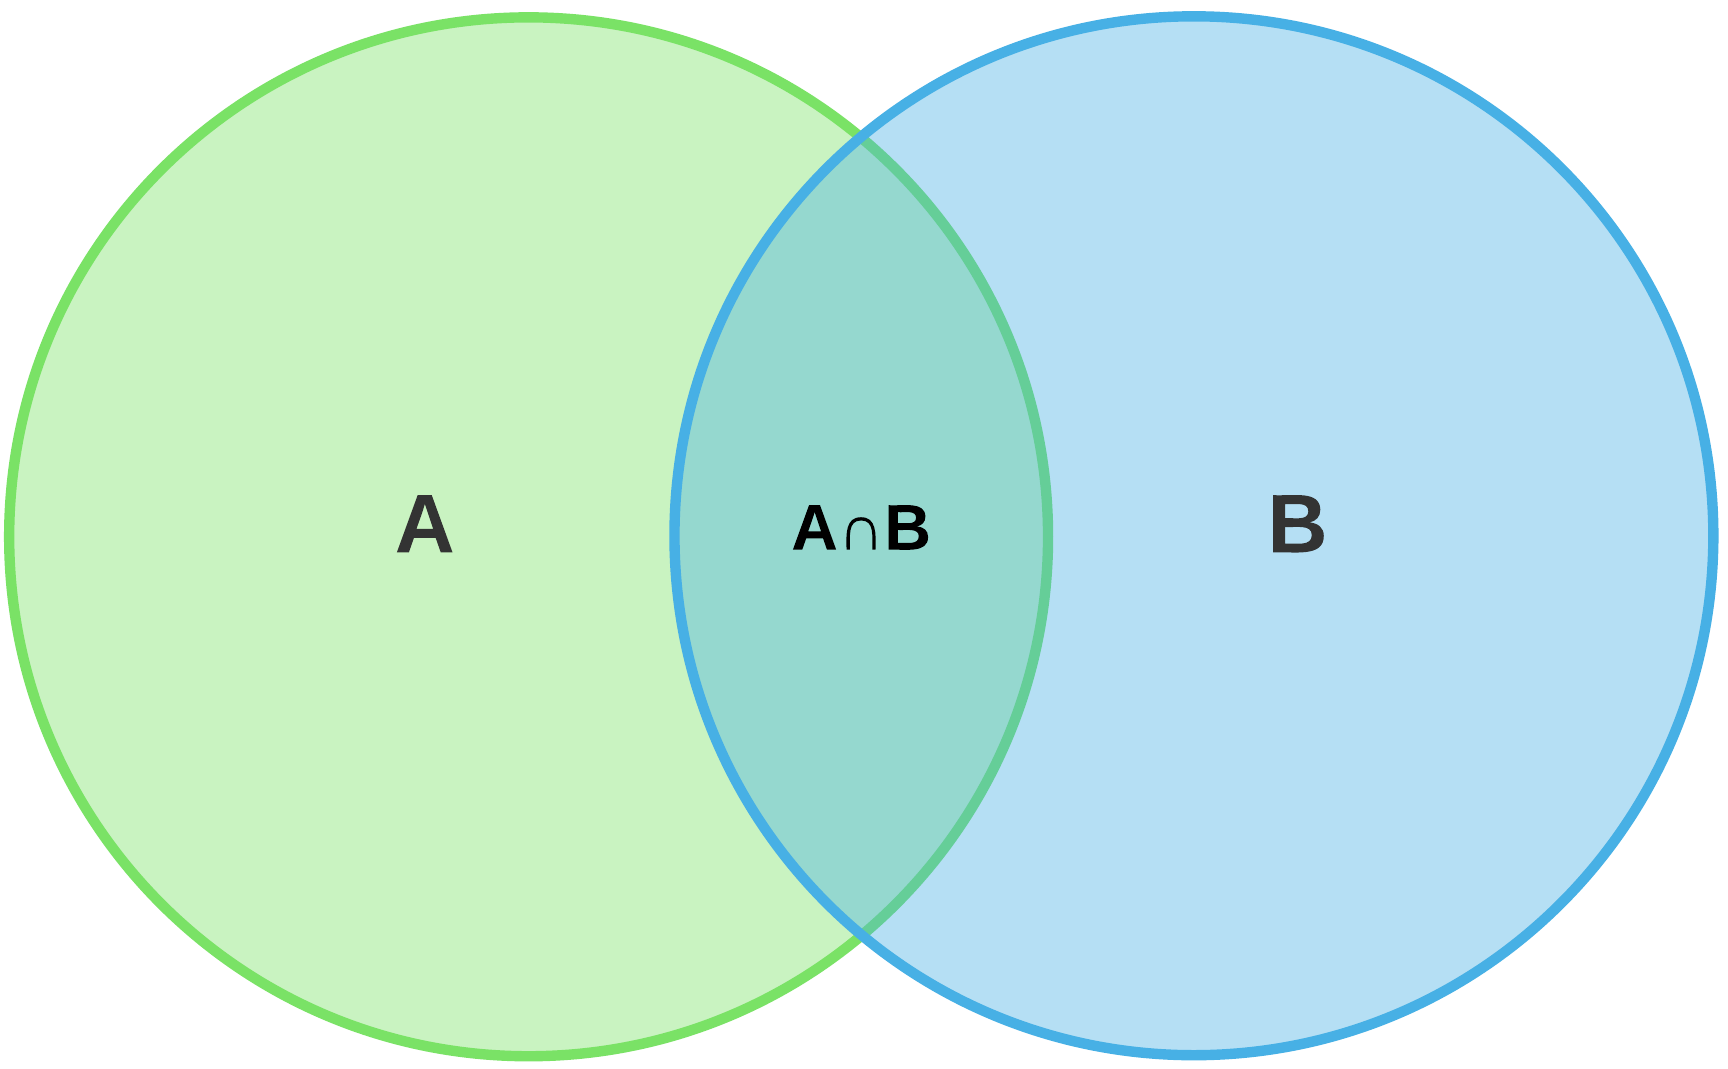
\includegraphics[width=0.5\textwidth]{img/venn.png}
    \caption{Events A and B}
    \label{fig:venn}
\end{figure}

\paragraph{Conditional probability rule:}
\begin{equation}
    P(B|A)=\frac{P(A\cap B)}{P(A)}=\frac{P(AB)}{P(A)}
\end{equation}

\paragraph{Multiplication rule:}
\begin{equation}
    P(AB)=P(B|A)\times P(A)
\end{equation}

\paragraph{Bayes Theorem:}
\begin{equation}
    P(A|B)=\frac{P(B|A)P(A)}{P(B)}; \qquad P(B)\neq 0
\end{equation}

\section{Distribution of Sample Mean}

The expected value (mean) and the variance of the sample mean ($X\sim N(\mu, \sigma^2)$) have the following expression
\begin{equation}
    \bar{X}=\frac{x_1+x_2+x_3+\ldots+x_n}{n}
\end{equation}
with mean
\begin{equation}
    \mu_{\bar{X}}=\mu
\end{equation}
and variance
\begin{equation}
    \sigma^2_{\bar{X}}=\frac{\sigma^2}{n}
\end{equation}

The standard deviation of the sampling distribution of $\bar{X}$, given by $\frac{\sigma}{\sqrt{n}}$ is called the \textbf{standard error}.

\textbf{Central Limit Theorem}: If $X_1,X_2,\ldots,X_n$ are a random sample of size $n$ taken from \textbf{ANY} unknown distribution (either finite/infinite) with mean $\mu$ and finite variance $\sigma^2$, then as $n$ gets larger the distribution of the sample mean $\bar{X}$ is approximately $N(\mu, \sigma^2/n)$

\section{Bayesian Analysis}
\paragraph{Prior:}
\begin{itemize}
    \item Frequentist inference assumes a fixed population parameter $\mu$.
    \item Bayesian inference places a distributional assumption on $\mu$ and treats $\mu$ as a random variable.
    \begin{equation}
        [\mu]\sim N(\mu_0, \tau^2)
    \end{equation}
    \item Distributional assumption on parameter is known as a prior. Prior parameters (e.g. $\mu_0$ and $\tau^2$) are known as hyper-parameters.
\end{itemize}

\paragraph{Likelihood:}
\begin{itemize}
    \item Let $\mathbf{y} = [y_1, y_2, \ldots, y_n]^T$ denote the vector of data, and the data likelihood is given by $[\mathbf{y}|\mu]$
\end{itemize}

\paragraph{Posterior distribution:}
\begin{itemize}
    \item $[\mu|\mathbf{y}]$ describes the probability distribution of $\mu$ based on the observed data.
    \item $[\mu|\mathbf{y}]$ can be calculated using the data likelihood $[\mathbf{y}|\mu]$ and the prior $[\mu]$.
    \begin{equation}
        [\mu|\mathbf{y}]=\frac{[\mathbf{y}|\mu]\times[\mu]}{[\mathbf{y}]} \propto [\mathbf{y}|\mu]\times[\mu]
    \end{equation}
    \item $[\mu|\mathbf{y}]$ is a distribution which we can make inference directly.
        \begin{itemize}
            \item 95\% Posterior interval: find constants $a$ and $b$ such that $P(a<\mu<b)=0.95$.
            \item Posterior hypothesis test: calculate $P(\mu>0)$.
        \end{itemize}
\end{itemize}

\paragraph{Unknown mean and variance:}
\begin{itemize}
    \item Priors: 
    \begin{equation}
        \mu\sim N(\mu_0, \tau^2); \quad \sigma^2\sim \operatorname{Inv-Gamma}(\alpha,\beta)
    \end{equation}
    \item Posterior distribution:
    \begin{equation}
        [\mu,\sigma^2|\mathbf{y}]=\frac{[\mathbf{y}|\mu,\sigma^2]\times[\mu]\times[\sigma^2]}{[\mathbf{y}]}
    \end{equation}
\end{itemize}

\paragraph{Bayesian Linear Regression:}
\begin{itemize}
    \item For a linear regression model with $(p+1)$ unknown parameters ($\beta_1, \beta_2, \ldots, \beta_p, \sigma^2$) and $n$ samples ($i=1,2,\ldots, n$):
        \begin{align}
            y_i=\beta_1x_{i1}+\beta_2x_{i2}+&\ldots+\beta_px_{ip}+\epsilon_i, \qquad \epsilon_i\sim N(0,\sigma^2) \\
            \mathbf{y}&\sim N(\bm{X\beta}, \sigma^2\mathbf{I}_{n\times n})
        \end{align}
    \item Priors:
        \begin{equation}
            \bm{\beta}\sim N(\bm{\mu_0}, \tau^2\mathbf{I}_{p\times p}); \quad \sigma^2\sim \operatorname{Inv-Gamma}(c_0,d_0)
        \end{equation}
\end{itemize}


\section{Meta Analysis}

Meta analysis is the statistical approach to combine information (statistical findings) from different sources.

\paragraph{Statistical model:}
\begin{itemize}
    \item Let $\hat{\beta_i}$ denote the estimated effect from study $i$ (\textit{e.g.,} log odds ratio, log relative risk, or regression coefficients). We assume
        \begin{equation}
            \hat{\beta_i}=\theta_i+\epsilon_i, \qquad \epsilon_i\sim N(0, \sigma^2_i)
        \end{equation}
        where $\theta_i$ is the unobserved true effect size and $\epsilon_i$ is the study-specific random deviation that is independent across studies with study specific variance $\sigma^2_i$.
\end{itemize}

\paragraph{Fixed effect model:}
\begin{itemize}
    \item This model assumes there is a single unknown parameter $\mu$ that each study is trying to estimate. If we assume $\theta_i=\mu$, then
        \begin{equation}
            \hat{\beta_i}=\mu+\epsilon_i, \qquad \epsilon_i\sim N(0, \hat{\sigma}^2_i)
        \end{equation}
    \item The optimal unbiased estimate for $\mu$ is
        \begin{equation}
            \hat{\mu}=\frac{\sum_{i=1}^n\hat{\beta}_i/\hat{\sigma}^2_i}{\sum_{i=1}^n1/\hat{\sigma}^2_i}
        \end{equation}
        a weighted average of $\hat{\beta}_i$ with inverse-variance as the weights.
\end{itemize}

\paragraph{Random effect model:}
\begin{itemize}
    \item Assuming $\theta_i$ are not all equal:
        \begin{equation}
            \hat{\beta_i}=\theta_i+\epsilon_i, \qquad \epsilon_i\sim N(0, \hat{\sigma}^2_i)
        \end{equation}
    \item Because we only observe one $\hat{\beta_i}$, we cannot estimate two parameters $\theta_i$ and $\epsilon_i$ jointly. One solution is to consider a second-level assumption on $\theta_i$:
        \begin{equation}
            \theta_i\sim N(\mu, \tau^2)
        \end{equation}
        We assume the unknown study-specific effect $\theta_i$ follows normal distribution with mean $\mu$ and variance $\tau^2$. $\mu$ is the overall pooled effect and $\tau^2$ is the between-study heterogeneity.
    \item It is natural to view the meta analysis model as a two-level normal random intercept model:
        \begin{align}
            &\hat{\beta_i}=\theta_i+\epsilon_i \\
            \theta_i\sim N(\mu, &\tau^2) \quad \epsilon_i\sim N(0, \hat{\sigma}^2_i)
        \end{align}
\end{itemize}

\paragraph{Bayesian Formulation:}
\begin{itemize}
    \item Data likelihood:
        \begin{align}
            &\hat{\beta_i}=\theta_i+\epsilon_i \\
            \theta_i\sim N(\mu, &\tau^2) \quad \epsilon_i\sim N(0, \hat{\sigma}^2_i)
        \end{align}
    \item Priors:
        \begin{align}
            &\mu\sim N(0, \nu_{\mu}^2) \\
            \tau^2\sim &\operatorname{Inv-Gamma}(a_0,b_0)
        \end{align}
\end{itemize}

%\bibliographystyle{plain}
%\bibliography{references}
\end{document}